% Classe do documento e parâmetros gerais.
\documentclass[report,a4paper,openright,twoside,11pt]{report}

% Packages utilizadas e respetivos parâmetros.
\usepackage[utf8]{inputenc}
\usepackage[english]{babel}
\addto{\captionsenglish}{\renewcommand{\bibname}{References}}
\addto{\captionsenglish}{\renewcommand{\contentsname}{Contents}}
\addto{\captionsenglish}{\renewcommand{\appendixname}{Appendix}}

\usepackage{lipsum} % gerador de texto
\usepackage{graphicx}
\usepackage{url}
\usepackage[Algoritmo]{algorithm}
\usepackage{algorithmicx}
\usepackage{algpseudocode}
\usepackage{hyperref}
\usepackage{listings}
\usepackage[
  list-style = table,         % lista em forma de tabela
  pages       = multiple      % recolhe todas as páginas de uso
]{acro}
\acsetup{make-links}
\renewcommand{\algorithmicrequire}{\textbf{Dados: }}
\renewcommand{\algorithmicensure}{\textbf{Resultado: }}

% Definições das dimensões das páginas
\setlength{\textheight}{24.00cm}
\setlength{\textwidth}{16cm}
\setlength{\topmargin}{0.35cm}
\setlength{\headheight}{0cm}
\setlength{\headsep}{0cm}
\setlength{\oddsidemargin}{0.25cm}
\setlength{\evensidemargin}{0.25cm}

%\renewcommand{\baselinestretch}{1}

% Declaração de acrónimos
\DeclareAcronym{bsc}{
  short=BSc,
  long=Bachelor of Science
}
\DeclareAcronym{api}{
  short=API,
  long=Aplication Programming Interface
}

\begin{document}
\pagenumbering{roman}
\thispagestyle{empty}

%=================== Página de título ===================
\begin{titlepage}
  \begin{center}
    \begin{minipage}[l]{\textwidth}
        \hspace{-15mm}\resizebox{85mm}{!}{
\includegraphics{../../img/figures/logoISELnew2.png}}\\
    \end{minipage}\\[10mm]
    {\large \textbf{Department of Electronical Engineering, Telecommunications and Computers}\\[1.5cm]}
    {\Huge \textbf{Remote Lab}\\[2cm]}    
    {\large \begin{tabular}{l}
      50565: Ângelo Azevedo \href{mailto:a50565@alunos.isel.pt}{(a50565@alunos.isel.pt)}\\
      50539: António Alves \href{mailto:a50539@alunos.isel.pt}{(a50539@alunos.isel.pt)}\\
    \end{tabular}\\[3cm] }
    {\large Report for Project and Seminar Class
    
    of Computer Science and Computer Engineering \acs{bsc}\\[3cm]}
    {\large Advisor: Prof. Pedro Miguens Matutino}   
    \vfill
    {\large \textbf{2 - 06 - 2025}}   
  \end{center}
\end{titlepage}

\baselineskip 18pt % line spacing: 12pt for single, 18pt for 1 1/2, and 24pt for double spacing

\newpage
\thispagestyle{empty}
% Fim da contracapa

% Página com identificação completa (número e nome) e assinaturas do(s) estudante(s) e do(s) orientador(es)
\cleardoublepage
\begin{center}
\textsc{\LARGE Lisbon School of Engineering}\\[15mm]

{\Large \bf  Remote Lab}\\[20mm]

\begin{tabular}{rl}
  50565  & Ângelo Azevedo\\[10mm]
           & \rule{75mm}{0.5pt}\\[5mm]

  50539  & António Alves\\[10mm]
           & \rule{75mm}{0.5pt}\\[5mm]

  Advisor: & Pedro Matutino\\[10mm]
      & \rule{75mm}{0.5pt}\\[5mm]
\end{tabular}\\[5cm]
{\large Report for Project and Seminar Class of Computer Science and Computer Engineering \acs{bsc}\\[3cm]}
June 2025\\
\end{center}

% Página de resumo em Inglês
\cleardoublepage
\chapter*{Abstract}
The design, development, implementation, and validation of digital systems require, in addition 
to simulators, the use of hardware for verification of their implementation in real devices. 
However, access to these real devices is sometimes restricted, not being available 24/7. 
In the current teaching paradigm where face-to-face time is reduced and remote and autonomous work 
is increased, it is necessary to create alternatives to the usual model.

The Remote Lab project aims to provide a virtual lab with access to remote hardware.
This lab consists of a web application running on an embedded system. The web application, accessed via a website, 
aims to provide a dashboard where users can join a laboratory. This
is where users can control the remote hardware. A hierarchy system will be implemented to
provide different roles, each with their own permissions relative to how users can browse the
information provided by the web application.

This project will implement the infrastructure to support the configuration, manipulation and visualization
of remote hardware. Based on an architecture with back-end (database and Web \acs{api}) and front-end (Web App, with a dashboard). 

\cleardoublepage
\chapter*{Resumo}
A conceção, desenvolvimento, implementação, e por fim a validação de sistemas digitais 
requerem para além dos simuladores, a utilização de hardware para uma verificação da sua 
concretização em dispositivos reais. No entanto, o acesso a esses dispositivos reais é por 
vezes restrito, não estando acessíveis 24h/7. No atual paradigma de ensino em que se reduz 
o tempo presencial, aumentando o trabalho remoto e autónomo, é necessário criar alternativas 
ao modelo habitual. 

O projeto Remote Lab tem como objetivo fornecer um laboratório virtual com acesso a hardware remoto.
Este laboratório consiste numa aplicação web executada num sistema embebido. A aplicação web, acedida 
através de um website, visa fornecer um dashboard onde os utilizadores podem aderir a um laboratório. 
É aqui que os utilizadores podem controlar o hardware remoto. Será implementado um sistema hierárquico para 
fornecer diferentes funções, cada uma com as suas próprias permissões relativamente à forma como os utilizadores 
podem navegar pela informação fornecida pela aplicação web.

Este projeto implementará a infraestrutura de suporte à configuração, manipulação e visualização de hardware remoto. 
Baseado numa arquitetura com back-end (base de dados e Web \acs{api}) e front-end (Web App, com um dashboard).

%{\bf Palavras-chave:} lista de palavras-chave separadas por ;.

%% Página de agradecimentos
%\cleardoublepage
%\chapter*{Agradecimentos}
%Texto dos agradecimentos. É opcional.\\

% Geração do índice de conteúdos
\tableofcontents 

% Geração do índice de figuras
\cleardoublepage
\phantomsection
\addcontentsline{toc}{chapter}{List of Figures}
\listoffigures

% Geração do índice de listas
\cleardoublepage
\phantomsection
\addcontentsline{toc}{chapter}{List of Listings}
\lstlistoflistings

% Geração do índice de acronyms
\cleardoublepage
\phantomsection
\addcontentsline{toc}{chapter}{Acronyms}
\printacronyms

% Reiniciar a numeração de páginas
\setcounter{page}{1}
\pagenumbering{arabic}

% Capitulo 1
%
% Chapter 1
%
\chapter{Introduction} \label{cap:intro}

%
% Secção 1.1
%
\section{Context and Motivation} \label{sec11}
In the recent years, the need for remote access to laboratory resources has grown significantly, driven by the expansion of online education, research collaboration, and the increasing complexity of experimental setups. Traditional laboratories often require physical presence, which can limit accessibility and flexibility for students, researchers, and professionals.
The \textbf{Remote Lab} here is proposed to address these challenges by providing a platform that enables secure, efficient, and user-friendly remote access to laboratory equipment and resources.

\section{State of the Art}

In recent years, several initiatives have emerged to provide remote access to laboratory resources, especially in the context of higher education and research. Projects such as \acs{mit}'s iLab~\cite{ilab} and LabShare~\cite{labshare} have demonstrated the feasibility and benefits of remote laboratories, enabling students and researchers to conduct experiments from anywhere in the world. These platforms typically focus on providing secure access, scheduling, and integration with a variety of laboratory equipment. The literature highlights the importance of usability, scalability, and security in the design of such systems, as well as the challenges associated with real-time interaction and hardware integration.

There are several systems that offer functionalities similar to those of the Remote Lab project. For example, the \acs{isa}, developed by \acs{mit}, is no longer operational and is not available for public access~\cite{ilab}. LabShare is another notable example, but it is currently also unavailable~\cite{labshare}. Other systems, such as WebLab-Deusto, focus on specific domains like electronics and instrumentation, providing specialized interfaces and tools for remote experimentation~\cite{weblabdeusto}. These systems serve as valuable references for the development of the Remote Lab platform, informing decisions related to architecture, user experience, and integration with laboratory hardware.

%
% Secção 1.2
%
\section{Objectives} \label{sec12}
The main objectives of the Remote Lab project are:
\begin{itemize}
    \item To design and implement a scalable platform for remote laboratory access.
    \item To ensure secure authentication and authorization for different user roles.
    \item To provide an intuitive user interface for managing and scheduling laboratory sessions.
    \item To support integration with various types of laboratory hardware.
\end{itemize}

This project focuses on the development of the core platform, including backend services, user management, and basic hardware integration. Advanced features such as real-time data analytics, support for a wide range of laboratory devices, and extensive reporting capabilities are considered out of scope for the current phase.

The project follows a modular and iterative development approach, leveraging modern software engineering practices. The backend is implemented using Kotlin and follows a layered architecture, while the frontend is developed with Next.js to provide a responsive and accessible user experience.

%
% Secção 1.3
%
\section{Structure of the Document} \label{sec13}
The structure of this report is as follows: Chapter 2 presents the related work, with a general overview of the existing solutions and technologies; Chapter 3 describes the system architecture; Chapter 4 details the main components and their interactions; Chapter 5 evaluates the system's performance and usability; and Chapter 6 presents the conclusions and future work perspectives.

% Capitulo 2
%
% Chapter 2
%
\chapter{Placement} \label{cap:placement}

This chapter is organized into two sections, where we describe related work and some systems similar to the one developed in this project.

\section{Related Work}
In recent years, several initiatives have emerged to provide remote access to laboratory resources, especially in the context of higher education and research. Projects such as MIT's iLab and LabShare have demonstrated the feasibility and benefits of remote laboratories, enabling students and researchers to conduct experiments from anywhere in the world. These platforms typically focus on providing secure access, scheduling, and integration with a variety of laboratory equipment. The literature highlights the importance of usability, scalability, and security in the design of such systems, as well as the challenges associated with real-time interaction and hardware integration.

\section{Similar Systems}
There are several systems that offer functionalities similar to those of the Remote Lab project. For example, the iLab Shared Architecture (ISA) provides a framework for sharing laboratory equipment over the internet, supporting both batch and interactive experiments. LabShare is another notable example, offering a collaborative platform for remote experimentation and resource sharing among institutions. Other systems, such as WebLab-Deusto and VISIR, focus on specific domains like electronics and instrumentation, providing specialized interfaces and tools for remote experimentation. These systems serve as valuable references for the development of the Remote Lab platform, informing decisions related to architecture, user experience, and integration with laboratory hardware.


% Capitulo 3
%
% Chapter 3
%
\chapter{Proposed Architecture} \label{cap:proposed-architecture}

This chapter presents the proposed architecture for the Remote Lab platform, detailing its main components, their interactions, and the rationale behind the architectural choices.

%
% Section 3.1
%
\section{System Overview} \label{sec31}
The Remote Lab platform is designed as a modular and scalable system, enabling secure and efficient remote access to laboratory equipment. The architecture follows a layered approach, separating concerns between the user interface, application logic, and hardware integration. This separation facilitates maintainability, extensibility, and the integration of new features or laboratory devices.

%
% Section 3.2
%
\section{Main Components} \label{sec32}
The architecture consists of the following main components:
\begin{itemize}
    \item \textbf{Frontend:} A web-based user interface developed with Next.js, providing users with access to laboratory resources, session scheduling, and experiment monitoring.
    \item \textbf{Backend:} Implemented in Kotlin, the backend exposes RESTful APIs for user management, authentication, authorization, and laboratory session control. It also handles business logic and enforces security policies.
    \item \textbf{Hardware Abstraction Layer:} This layer manages communication with laboratory equipment, abstracting hardware-specific details and providing a unified interface for the backend.
    \item \textbf{Database:} Stores user data, session information, access logs, and configuration settings. The database ensures data consistency and supports auditing requirements.
    \item \textbf{Authentication and Authorization:} Ensures secure access to the platform, supporting multiple user roles (e.g., students, professors, administrators) with different permissions.
\end{itemize}

%
% Section 3.3
%
\section{Component Interactions} \label{sec33}
The components interact as follows:
\begin{itemize}
    \item Users interact with the frontend to authenticate, schedule sessions, and access laboratory resources.
    \item The frontend communicates with the backend via secure API calls.
    \item The backend processes requests, applies business logic, and interacts with the database and hardware abstraction layer as needed.
    \item The hardware abstraction layer translates backend commands into device-specific instructions, enabling remote control of laboratory equipment.
\end{itemize}

%
% Section 3.4
%
\section{Architecture Diagram} \label{sec34}
Figure~\ref{fig:architecture} illustrates the high-level architecture of the Remote Lab platform.

% Insert architecture diagram here
\begin{figure}[h]
\begin{center}
    \resizebox{100mm}{!}{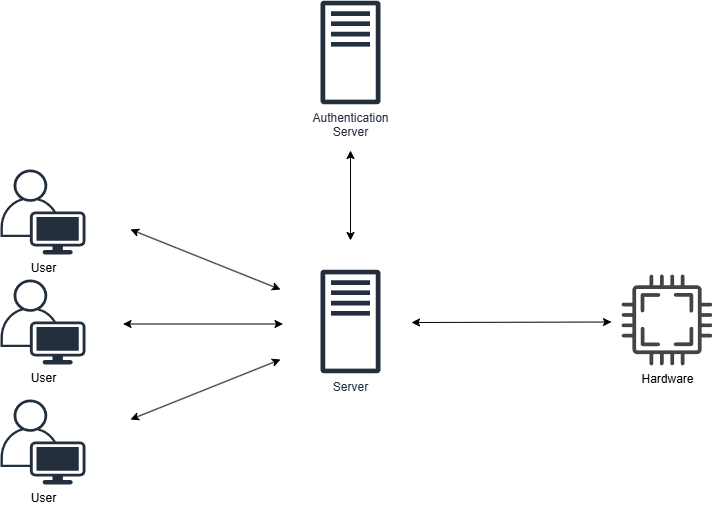
\includegraphics{./../img/SimpleArchitectureRL.drawio.png}}
\end{center}
\caption{High-level architecture of the Remote Lab platform.}\label{fig:architecture}
\end{figure}

%
% Section 3.5
%
\section{Design Rationale} \label{sec35}
The architectural choices were guided by the need for scalability, security, and ease of integration with diverse laboratory equipment. The use of a layered architecture and standardized interfaces ensures that the platform can evolve to meet future requirements and support additional functionalities.

% Capitulo 4
%
% Chapter 4
%
\chapter{Implemented Infrastructure} \label{cap:implemented-infrastructure}

This chapter details the infrastructure implemented for the Remote Lab platform, covering the main components, technologies, deployment strategy, and integration between system modules.

\section{Overview}

The Remote Lab platform is designed as a modular, containerized system that enables secure and efficient remote access to laboratory equipment. The infrastructure follows a layered architecture, separating the user interface, backend logic, and hardware integration, and is built with scalability and maintainability in mind.

\begin{figure}[h]
    \begin{center}
        \resizebox{16cm}{!}{\includesvg{../img/SystemArchitectureWithTechRL.svg}}
    \end{center}
    \caption{System Architecture Overview}
    \label{fig:system-architecture}
\end{figure}

\section{Project Structure}

The Remote Lab project is organized into several main directories, each of which is managed as a GitHub submodule. This approach allows for independent development, versioning, and access control of each core component, supporting both modularity and security. The use of submodules also facilitates collaboration among different teams and ensures that sensitive information is handled appropriately.

The main submodules of the project are:

\begin{itemize}
    \item \textbf{api/} -- Contains the backend source code, implemented in Kotlin with Spring Boot. This submodule is responsible for business logic, user management and laboratory session control.
    \item \textbf{db/} -- Includes database scripts, supporting the persistence layer of the system.
    \item \textbf{docs/} -- Stores project documentation, including technical reports, user guides, and architectural diagrams.
    \item \textbf{img/} -- Stores project images, including diagrams, screenshots, and other visual representations of the system.
    \item \textbf{nginx/} -- This directory is not a GitHub submodule but it provides Nginx configuration files for reverse proxying, load balancing, and secure access to backend services.
    \item \textbf{private/} -- Dedicated to sensitive files and configurations, such as environment variables and secrets necessary for the secure operation of the system, and specific to our implementation choices. This submodule contains the information and configuration files required to run the project with our selected authentication (login) and database setup, reflecting the particular options chosen for our use case. It is not included directly in the main repository, ensuring that only authorized members have access to confidential information like API keys, external service credentials, and other private data essential for both production and development environments.
    \item \textbf{website/} -- Holds the frontend web application, built with Next.js (React). This submodule provides the user interface for laboratory access, scheduling, and management.
    \item \textbf{wiki/} -- Stores the GitHub Wiki pages, including the project documentation, deployment instructions, and other relevant information.
\end{itemize}

This modular structure, based on GitHub submodules, allows for independent development, testing, and deployment of each component, supporting both scalability and maintainability. By clearly separating concerns and leveraging best practices such as containerization and secure secret management, the project is well-positioned for collaborative development and future expansion. 

\section{Implementation Details}

Key implementation decisions and details include:

\begin{itemize}
    \item \textbf{Containerization:} All major components (frontend, backend, database) are containerized using Docker, ensuring consistent environments across development and production.
    \item \textbf{Orchestration:} Docker Compose is used to manage multi-container deployments, networking, and environment configuration.
    \item \textbf{Backend:} The backend uses JDBI for type-safe database access and is configured via environment variables for flexibility and security.
    \item \textbf{Frontend:} The frontend is built with Next.js, providing a modern, responsive interface and integrating with the backend via RESTful APIs.
    \item \textbf{Authentication:} Microsoft OAuth (via NextAuth) is used for secure authentication, enabling university login. The system is designed to be flexible, so other OAuth providers or even an internal login mechanism could be used if required.
    \item \textbf{Role-based Access Control:} The system enforces permissions based on user roles, ensuring secure and appropriate access to resources.
    \item \textbf{Hardware Abstraction:} The backend abstracts hardware-specific details, allowing for easy extension to new laboratory equipment.
    \item \textbf{Automation:} The \texttt{start.sh} script automates the bootstrap process, starting all necessary services with a single command.
\end{itemize}

\subsection*{Role-Based Access Control (RBAC)}

The system implements Role-Based Access Control (RBAC) to ensure that users have access only to the resources and actions appropriate for their role. Each authenticated user is assigned a role, such as student, professor, or administrator, which determines their permissions within the platform. 

Roles are enforced both on the backend and frontend. On the backend, endpoints and business logic check the user's role before allowing access to sensitive operations, such as managing laboratory sessions, accessing administrative features, or modifying user data. On the frontend, the user interface dynamically adapts to the user's role, displaying only the features and options relevant to their permissions.

The main roles in the system are:
\begin{itemize}
    \item \textbf{Student:} Can view and book laboratory sessions, access their own session history, and interact with laboratory equipment during their reserved times. Students have access only to features relevant to their participation in laboratory activities.
    \item \textbf{Professor:} In addition to all student permissions, professors can create and manage laboratory sessions, view and manage student participation, and access additional data and reports related to their classes or laboratories.
    \item \textbf{Administrator:} Has full access to all system features, including user management, system configuration, and oversight of all laboratory sessions and resources. Administrators can manage roles, permissions, and perform maintenance or troubleshooting tasks across the platform.
\end{itemize}

This approach provides a secure and flexible way to manage access, making it easy to introduce new roles or adjust permissions as the platform evolves. The RBAC system is central to maintaining the integrity and security of the Remote Lab environment.

These choices ensure the platform is robust, extensible, and easy to deploy or develop locally.

In addition, the web application allows users to view and interact with the platform as if they had a lower role than their own. This feature is particularly useful for testing, support, and understanding the user experience from different perspectives. For example, an administrator or professor can switch to a student view to verify permissions, troubleshoot issues, or provide guidance, without needing to log in as a different user. 

\section{Database}
The database serves as the foundational component of the system architecture. PostgreSQL was selected as the database management system due to its reliability, open-source nature, and robust support for relational data models. This choice aligns with previous project implementations and provides the consistency and performance required for the system's operational needs.

This section presents a overview of the \ac{er model} and critical implementation details. Complete technical documentation is provided in the accompanying appendix.

\subsection{Entity-Relationship Model}

\begin{figure}[H]
    \begin{center}
        \resizebox{17cm}{!}{\includesvg{../img/DB-diagrams/ERDiagramRL.svg}}
    \end{center}
    \caption{Entity-Relationship Model (ER Model)}
    \label{fig:er_model}
\end{figure}

The database design follows a normalized relational structure that supports user authentication, secure session management, and the remaining system functionalities. The ER model encompasses the core entities required for system functionality while maintaining data integrity and scalability.

\subsection*{Core Entities}
\subsection*{User}

\begin{figure}[H]
    \begin{center}
        \resizebox{10cm}{!}{\includesvg{../img/DB-diagrams/User.svg}}
    \end{center}
    \caption{User Entity}
    \label{fig:user_entity}
\end{figure}

The \textbf{User} entity represents a user in the system. The username and email attributes are provided by the authentication system. The role serves as descriminator attribute to identify whether the user is an administrator, professor or student.

\subsection*{Token}

\begin{figure}[H]
    \begin{center}
        \resizebox{10cm}{!}{\includesvg{../img/DB-diagrams/Token.svg}}
    \end{center}
    \caption{Token Entity}
    \label{fig:token_entity}
\end{figure}

A user can create \textit{N} tokens. The \textbf{Token} is a weak entity because it cannot be identified by its attributes alone and therefore requires a user, which is a strong entity, to be identified. Its attributes cannot uniquely identify it. A token is created by only one user.

This is a useful entity for authentication propuses. It was designed to hold a hash value in the \textit{token\_validation} attribute.

Authentication workflow:

\begin{enumerate}
    \item Upon successful user login, a unique token is created with cryptographically secure values and stored in the database.
    \item For subsequent authenticated operations, the system queries the database to verify the client-provided token against stored values.
    \item Valid tokens enable secure user identification without transmitting unique identifiers.
\end{enumerate}

The \textit{last\_used\_at} and the \textit{created\_at} are useful for determining token expiration.

\subsection*{Laboratory}

\begin{figure}[H]
    \begin{center}
        \resizebox{10cm}{!}{\includesvg{../img/DB-diagrams/Laboratory.svg}}
    \end{center}
    \caption{Laboratory Entity}
    \label{fig:laboratory_entity}
\end{figure}

A user, as an administrator or professor, can create \textit{N} laboratories. When creating a \textbf{Laboratory}, the user can define the name (\textit{lab\_name}) and description (\textit{lab\_description}). They can also define the duration of a laboratory session (\textit{lab\_duration}) and its queue limit (\textit{lab\_queue\_limit}).

\subsection*{Hardware}

\begin{figure}[H]
    \begin{center}
        \resizebox{10cm}{!}{\includesvg{../img/DB-diagrams/Hardware.svg}}
    \end{center}
    \caption{Hardware Entity}
    \label{fig:hardware_entity}
\end{figure}

Upon successful laboratory creation, the user can associate \textbf{Hardware} to it, which must be created separately.

For the creation, it requires a name (\textit{hw\_name}), IP (\textit{ip\_address}) and MAC (\textit{mac\_address}) addresses (which can be null depending on the hardware), a status (\textit{hw\_status}) to indicate whether the hardware is under maintenance, occupied, or available, and a serial number (\textit{hw\_serial\_num}) to uniquely identify the hardware. Although it has an ID, the serial number helps physically identify the hardware.    

\subsection*{Group}

\begin{figure}[H]
    \begin{center}
        \resizebox{9cm}{!}{\includesvg{../img/DB-diagrams/Group.svg}}
    \end{center}
    \caption{Group Entity}
    \label{fig:group_entity}
\end{figure}

For a student to access a laboratory, they must be in a group that is associated with that laboratory. A professor can create a \textbf{Group} and associate users to it.

When creating a group, the user needs to name it (\textit{group\_name}) and, optionally, add a description (\textit{group\_description}) to it.

\subsection*{Lab Session}

\begin{figure}[H]
    \begin{center}
        \resizebox{7.5cm}{!}{\includesvg{../img/DB-diagrams/LabSession.svg}}
    \end{center}
    \caption{Lab Session Entity}
    \label{fig:lab_session_entity}
\end{figure}

Finally, a user can join a laboratory if they are in a group associated with it. If the laboratory is being used, the user enters a waiting queue; otherwise, a \textbf{Lab Session} is created.

Lab Session is a weak entity. It requires two strong entities to be identified: the \textbf{User} entity and the \textbf{Laboratory} entity. This is used to check whether a user is in a lab session or for statistical purposes. The \textit{state} attribute indicates whether the session is over or still running. The \textit{start\_time} and \textit{end\_time} can be used for statistical details, such as determining how much time a user spent in a laboratory, or for future purposes, such as scheduling sessions.

\subsection{Implementation Details}
After providing an overview of the database entities and their associations, there are important details worth mentioning:

\begin{itemize}
    \item Although PostgreSQL is being used for its functionalities, it was decided that all logic and verifications are implemented in the Web API, so that no triggers or complex constraints are implemented on the database side.
\end{itemize}

\subsection{Conclusion}
This section has provided an overview of the database architecture, implementation, and design decisions. It has also presented the \acs{er model} of the database and described a typical user journey, explaining database interactions.

The documentation should be consulted for a comprehensive deep dive. It explains every entity, its attributes, and provides theoretical insights.

\section{Web API}
The Web API provides endpoints for user management, authentication, authorization, and CRUD operations. 

The API is developed with Kotlin and Spring Boot, and follows the Controller-Service-Repository pattern, which is prevalent in many Spring Boot applications. We chose this pattern because of the separation of concerns it provides and the possibilities for unit testing.

To make the codebase even easier to maintain and improve the quality of life during development, Spring Framework's Inversion of Control container (COLOCAR REFERENCIA) and the Strategy pattern principle were also used. 

Spring's dependency injection is a well-known technology in Java enterprise programming. It provides an easy way to declare dependencies, since the API was mostly built following Object Oriented Programming (OOP) principles. This framework allows us to declare the necessary dependencies for each module. It also provides a BeanFactory interface for advanced configurations. Using these Spring technologies moves the object management to Spring.

The Strategy pattern allowed us to have more control over the specific implementation since it follows an interface. Every concrete implementation follows an interface, making it possible to change a class dynamically without changing the code. Spring's dependency injection works very well with this strategy design pattern. This makes unit tests much easier when the concrete implementation is not intended to be tested without changing it's code.

\begin{figure}[H]
    \begin{center}
        \resizebox{15cm}{!}{\includesvg{../img/api/api_architecture.svg}}
    \end{center}
    \caption{API Architecture}
    \label{fig:api_architecture}
\end{figure}

Figure \ref{fig:api_architecture} provides a simple overview of the implemented \acs{api}. The \textbf{HTTP} module (Controller) is responsible for exposing the endpoints and handling the messages. When a request is made, the HTTP module receives the request and hands it to the \textbf{Service} module. This is where the logic and verifications are performed. Since it is necessary to fetch and save data, a \textbf{Repository} module is needed. The repository module is responsible for communicating with the database.

\vspace{3mm}

\begin{figure}[H]
    \begin{center}
        \resizebox{15cm}{!}{\includesvg{../img/api/detailed_architecture.svg}}
    \end{center}
    \caption{API Detailed Architecture}
    \label{fig:api_detailed_architecture}
\end{figure}

Figure \ref{fig:api_detailed_architecture} provides a more detailed overview of how the architecture is composed. 

As explained, the HTTP module contains the controllers, each one with its functions. The pipeline contains the argument resolvers and interceptors. For the implemented system, only one argument resolver and two interceptors were implemented. The argument resolver (COLOCAR REFERENCIA) is used to provide user information to the controllers. Since the authentication method we used was token-based, this argument resolver extracts user information from the request. Every controller that has a parameter with the type \textit{AuthenticatedUser} will be authenticated. 

For the request to contain the needed information about the user, an interceptor is required. This is one of the two interceptors implemented. Every request, before reaching the controller, passes through every configured interceptor. This authentication interceptor checks if the handler parameters contain a parameter of the type \textit{AuthenticatedUser}. If it does, the entire process of getting the token from the request, verifying it, and retrieving the user is performed. If not, normal execution continues.
\begin{center}
    \begin{lstlisting}[caption={Type AuthenticatedUser verification example}]
    if (handler is HandlerMethod &&
        handler.methodParameters.any {
            it.parameterType == AuthenticatedUser::class.java
        }
    )
    \end{lstlisting}
\end{center}

The other interceptor is for an API key. It checks if the handler contains a custom annotation. If yes, the API key is validated; if not, an unauthorized response is sent. This interceptor is useful for the login endpoint. This login endpoint is to be performed in the Web App and is not meant to be used by end users.

The service module performs the necessary checks, using domain classes defined in the Domain module. These classes provide configurations and methods for validating certain data. Configurations in domain classes are provided by a JSON file containing domain restrictions.

\begin{center}
    \begin{lstlisting}[caption={Example of the group entry}]
        "group": {
            "groupName": {
              "min": 3,
              "max": 100,
              "optional": false
            },
            "groupDescription": {
              "min": 10,
              "max": 1000,
              "optional": true
            }
          }
    \end{lstlisting}
\end{center}

This JSON file is converted to a class using Kotlin Serialization. This allows an easy way to change specific values without touching the codebase.

\vspace{3mm}

Every response, whether successful or an error, follows a specific format. The API documentation provides an overview of the possible responses. Error messages follow the application/problem+json format (COLOCAR REFERENCIA).

\vspace{3mm}

The API is expected to be public, providing full documentation (COLOCAR REFERENCIA POSTMAN) in Postman. It was decided to have the documentation in Postman because of the easy-to-use documentation builder inside the collection containing the tests for the endpoints. The API key is implemented for this reason. In future work, when the API reaches a stable version to be made public, users who want to use it will need to log in to the website and generate a token to use the API.

\section{Web Application}



\section{Deployment}

The deployment process for the Remote Lab platform is designed to be straightforward, secure, and reproducible, leveraging modern DevOps practices and containerization technologies.

\subsection{Containerization and Orchestration}
All major components of the platform—including the backend (api), frontend (website), and database—are containerized using Docker. This ensures consistency across development, testing, and production environments. Docker Compose is used to orchestrate multi-container deployments, manage networking between services, and handle environment-specific configurations.

\subsection{Environment Configuration and Secrets}
Sensitive configuration files and environment variables required for deployment are managed in the \textbf{private/} submodule. This submodule contains the necessary secrets, such as API keys, database credentials, and authentication settings, tailored to the specific requirements of the platform. Access to this submodule is restricted to authorized team members, ensuring the security of confidential information.

\subsection{Automation with start.sh}

To further streamline the deployment process, the platform provides a \texttt{start.sh} script located at the root of the repository. This script automates the bootstrap process by orchestrating the initialization of all required services and dependencies with a single command. It handles tasks such as building Docker images, starting containers using Docker Compose, and ensuring that environment variables and configuration files are correctly loaded from the \texttt{private/} submodule.

The \texttt{start.sh} script also supports several flags to customize the deployment process, such as selecting the environment (development or production), starting only the API, enabling Cloudflare tunneling, or switching branches. These options make it easy to adapt the deployment to different scenarios with simple command-line arguments.

\subsection{Deployment Steps}
\begin{enumerate}
    \item \textbf{Clone the Repository and Submodules:} Clone the main repository and initialize all submodules, including \texttt{private/}, to ensure all components and configurations are available.
    \item \textbf{Configure Environment Variables:} Ensure that all required environment variables and secret files are present in the appropriate locations, as provided by the \texttt{private/} submodule.
    \item \textbf{Build and Start Services:} Use the provided \texttt{docker-compose.yml} file to build and start all services with a single command (e.g., \texttt{docker compose up --build}).
    \item \textbf{Access the Platform:} Once all containers are running, the platform can be accessed via the configured web address. Nginx is used as a reverse proxy to route traffic securely to the appropriate services.
\end{enumerate}

\subsection{Local and Production Deployment}
The deployment process is designed to be nearly identical for both local development and production environments. Developers can run the entire stack locally using Docker Compose, mirroring the production setup. For production, additional considerations such as SSL certificates, domain configuration, and scaling may be applied, but the core process remains the same.

This approach ensures that deployments are reliable, repeatable, and secure, minimizing the risk of configuration drift and simplifying both initial setup and ongoing maintenance.


\section{Technologies Used}

\begin{itemize}
    \item \textbf{Frontend:} Implemented with Next.js (React framework), providing a modern, responsive web interface for users to interact with laboratories, schedule sessions, and control hardware.
    \item \textbf{Backend:} Developed in Kotlin using Spring Boot, exposing RESTful APIs for user management, authentication, laboratory session control, and business logic enforcement.
    \item \textbf{Database:} PostgreSQL is used to persist user data, session information, access logs, and configuration settings.
    \item \textbf{ORM/Database Access:} JDBI is used for type-safe, modular database access in the backend.
    \item \textbf{Authentication:} Microsoft OAuth via NextAuth is used for user authentication, supporting multiple roles (student, professor, administrator).
    \item \textbf{Containerization:} Docker is used to containerize all major components (frontend, backend, database), ensuring consistent deployment across environments.
    \item \textbf{Orchestration:} Docker Compose manages multi-container deployment, networking, and environment configuration.
\end{itemize}

\section{System Components}

\begin{itemize}
    \item \textbf{Web Application (Frontend):} Provides dashboards, laboratory access, real-time hardware monitoring, and session management. Built with Next.js and deployed as a Docker container.
    \item \textbf{API Server (Backend):} Handles authentication, authorization, laboratory and user management, and hardware abstraction. Built with Kotlin and Spring Boot, also containerized.
    \item \textbf{Database:} PostgreSQL instance running in a Docker container, with persistent storage volumes.
    \item \textbf{Hardware Abstraction Layer:} Backend modules abstract hardware-specific details, exposing unified interfaces for laboratory equipment control.
\end{itemize}

\section{Deployment Architecture}

The system is deployed using Docker Compose, which defines and manages the following services:

\begin{itemize}
    \item \textbf{db:} PostgreSQL database container, with health checks and persistent volumes.
    \item \textbf{api:} Backend API container, built from the Kotlin/Spring Boot project, depending on the database service.
    \item \textbf{website:} Frontend container, built from the Next.js project, depending on the API service.
\end{itemize}

All services are connected via Docker networks to ensure secure and efficient communication. Environment variables and secrets are managed via \texttt{.env} files.

\section{Build and CI/CD}

\begin{itemize}
    \item \textbf{Gradle:} Used for building and managing backend dependencies.
    \item \textbf{NPM:} Used for frontend dependency management and builds.
    \item \textbf{Dockerfiles:} Multi-stage builds are used for both backend and frontend to optimize image size and security.
    \item \textbf{GitHub Actions:} (If applicable) Used for continuous integration and automated builds.
\end{itemize}

\section{Notable Implementation Details}

\begin{itemize}
    \item The backend uses JDBI for database access, configured with application-specific requirements.
    \item Environment variables are used to configure database connections and secrets, improving security and flexibility.
    \item The system supports role-based access control, with different permissions for students, professors, and administrators.
    \item The hardware abstraction layer allows for future extension to new types of laboratory equipment.
\end{itemize}

\section{Summary}

The implemented infrastructure leverages modern web technologies, containerization, and modular design to provide a robust, scalable, and maintainable platform for remote laboratory access.
%\chapter{Exemplos} \label{cap:exemplos}

A nossa solução é apresentada neste capítulo. A solução consiste em grandes ideias, desenvolvidas e testadas.

Exemplo de indentação do segundo parágrafo.

\section{Nome da primeira secção deste capítulo} \label{sec31}
Texto da secção. Seguem-se exemplos de vários parágrafos.

Esta unidade curricular funciona no semestre de Verão de cada ano letivo. Nos casos de impedimento prolongado justificado (designadamente por doença ou por motivos profissionais no caso dos trabalhadores-estudantes), poderá ser prolongada, havendo lugar à elaboração de outro relatório de progresso
e a nova inscrição se o prolongamento for além do período de época especial desse semestre. A entrega da justificação e a sua apreciação deverão ocorrer antes do final do prazo estabelecido para a entrega final.

O estudante só poderá frequentar Projecto e Seminário se, em conjunto com as restantes unidades curriculares em que se inscreve nesse semestre isso corresponder, no máximo, a 44 créditos ECTS, tendo acumulado, pelo menos, 138 créditos. No caso de estudantes em regime de tempo parcial, o valor máximo
está limitado a 30 créditos no ano letivo. Não são admitidas inscrições como unidade curricular isolada.

Anualmente é divulgada a lista de ideias para projetos e respetivos orientadores. Os estudantes poderão propor outras ideias identificando os orientadores. A escolha da ideia de projeto é feita no período de
interrupção letiva após o semestre de Inverno. As propostas de projeto são registadas no início do período letivo do semestre de Verão, verificado que os estudantes reúnem as condições de frequência.
O projeto deve ser realizado em grupo de dois estudantes (excecionalmente um ou três). Cada elemento do grupo tem tarefas específicas pelas quais é responsável. Esta situação deve ficar clara desde o início do projeto.

A orientação dos projetos é feita por docentes da área departamental onde o curso está ancorado ou por especialistas externos, podendo haver coorientadores, mas sendo obrigatória a coorientação por docente da área departamental no caso de orientação externa. O desenvolvimento do projeto é acompanhado de reuniões periódicas do orientador (ou coorientadores) com o grupo. A informação referente ao projeto é mantida em formato eletrónico em local acessível pelos elementos do grupo, pelos orientadores e pelos docentes de Projecto e Seminário.\\

A avaliação de Projecto e Seminário envolve:
\begin{enumerate}
	\item proposta do projeto;
	\item relatório de progresso;
	\item apresentação individual;
	\item cartaz e versão beta do projeto;
	\item relatório de projeto e discussão pública final.
\end{enumerate}

A avaliação incide sobre o trabalho planeado e desenvolvido pelos estudantes, com constrições de tempo e prazos previamente estabelecidos. Se durante a realização do projeto for considerado que este está em risco, ouvidos os estudantes envolvidos, o orientador e o docente da unidade curricular decidem se o projeto continua. Em caso de desistência do estudante, esta deve ser comunicada ao orientador do projeto e ao regente da unidade curricular.

\section{A segunda secção deste capítulo} \label{sec32}
Na segunda secção deste capítulo, vamos abordar o enquadramento,
o contexto e as funcionalidades.

\subsection{A primeira sub-secção desta secção} \label{sec321}
As sub-secções são úteis para mostrar determinados conteúdos de forma
organizada. Contudo, o seu uso excessivo dificulta a leitura do documento.

\subsection{A segunda sub-secção desta secção} \label{sec322}
Esta é a segunda sub-secção desta secção, a qual termina aqui.

\section{Descrição detalhada da solução} \label{sec33}
A solução proposta assenta nas seguintes ideias. O algoritmo~\ref{alg1}
apresenta as ações de pesquisa de um elemento $E$ sobre um grafo $G$.
\begin{algorithm}
\caption{Algoritmo de pesquisa em grafo.}
\label{alg1}
\algorithmicrequire{Grafo G, Elemento E}\\
\algorithmicensure{Localização de E em G}\\
\begin{enumerate}
\item Para todos os vértices $v$ em $G$
\item Pesquisar e obter a localização de $E$
\begin{enumerate}
	\item Iniciar a lista de pontos, $P$
	\item Ordenar $P$
\end{enumerate}	
\end{enumerate}
\end{algorithm}

\newpage
Nalgumas situações, é necessário apresentar excertos de
código que ilustrem aspetos relevantes da implementação.

\begin{verbatim}
namespace ps;
public static void main() {
		System.out.println(``PS - Projecto e Seminário'');
}
\end{verbatim}

% Capitulo 4
%\chapter{Testes} \label{cap:testes}

Este é o capítulo de testes. 
É possível forçar a inclusão de todas as referências com \cite{*}.

Modo de matemática em texto $x = ma^2$ e em equação (duas formas):
\[
    x = ma^2
\]

\begin{equation}
    x = ma^2
\end{equation}

% Referências
\bibliographystyle{unsrt}
\bibliography{references}
\addcontentsline{toc}{chapter}{References}

% Apêndices (opcional)
%\appendix
%%
% Apêndice 1
%
\chapter{Exemplo de apêndice} \label{ap:exemplo}
Este é o primeiro parágrafo do apêndice.


\lipsum[14-16]

\end{document}